\begin{enumerate}

\item A car has two wipers which do not overlap. Each wiper has a blade of length $21 \mathrm{cm}$ sweeping through an angle of $120\degree$. Find the total area cleaned at each sweep of the two blades.

\item Sides $AB$ and $BC$ and median $AD$ of a triangle $ABC$ are respectively proportional to sides $PQ$ and $QR$ and median $PM$ of $\triangle PQR$.Show that $\triangle ABC \sim \triangle PQR$.

\item Through the mid-point $M$ of the side $CD$ of a parallelogram $ABCD$,the line $BM$ is drawn intersecting $AC$ in $L$ and $AD$ (produced) in $E$.Prove that $EL = 2BL$. 

\item In the given figure, $O$ is the center of the circle .$AB$ and $AC$ are tangents drawn to the circle from point $A$. If $\angle BAC = 65\degree $, then find the measure of $\angle BOC $.
	\begin{figure}[!ht]
		\centering
		\includegraphics[width=\columnwidth]{figs/last5.jpg}
		\caption{}
		\label{fig:enter-label}
	\end{figure}

\newpage
\item In the given figure, $O$ is the centre of the circle and $QPR$ is a tangent to it at $P$.Prove that $\angle QAP + \angle APR = 90\degree$.

	\begin{figure}[!ht]
		\centering
		\includegraphics[width=\columnwidth]{figs/last4.jpg}
		\caption{}
		\label{fig:enter-label}
	\end{figure}
\newpage
\item In an annual day function of a school, the organizers wanted to give a cash prize along with a memento to their best students.Each memento is made as shown in the figure and its base $ABCD$ is shown from the front side.The rate of silver plating \rupee~20 $per  \mathrm{cm}^2$.

	\begin{figure}[!ht]
		\centering
		\includegraphics[width=\columnwidth]{figs/last3.jpg}
		\caption{}
		\label{fig:enter-label}
	\end{figure}

	\text Based on the above, answer the following question:
		\begin{enumerate}
			\item What is the area of the quadrant $ODOC$?
			\item Find the area of $\triangle AOB$.
			\item
			\begin{enumerate}
				\item What is the total cost of silver plating the shaded part $ABCD$?
				\item What is the length of arc $CD$ ?
			\end{enumerate}
		\end{enumerate}
\newpage
\item In a coffee shop, coffee is served in two types of cups.One is cylindrical  in shape with diameter $7 \mathrm{cm}$ and height $14 \mathrm{cm} $ and the other is hemispherical with diameter $21 \mathrm{cm}$.

	
	\begin{figure}[!ht]
		\centering
		\includegraphics[width=\columnwidth]{figs/last2.jpg}
		\caption{}
		\label{fig:enter-label}
	\end{figure}

	\text Based on the above, answer the following question:
	\begin{enumerate}
		\item  Find the area of the cylindrical cup.
		\item
		\begin{enumerate}
			\item  What is the capacity of the hemispherical cup?
			\item Find the capacity of the cylindrical cup.
		\end{enumerate}
		\item   What is the curved surface area of the cylindrical cup?
         \end{enumerate}

\newpage	
\item Show that the points $\brak{-2,3}, \brak{8,3}$ and $\brak{6,7} $ are the vertices of a right-angled triangle.

\item If $Q\brak{0,1}$ is equidistant from $P\brak{5,-3}$ and $R\brak{x,6}$,find the values of $x$.
\item In the given figure, $TA$ is a tangent to the circle with center $O$ such that $OT = 4\mathrm{cm}$, $\angle OTA = 30\degree$, then the length of $TA$ is:
    \begin{enumerate}
        \item $2 \times \sqrt{3} \mathrm{cm}$
        \item $2\mathrm{cm}$
        \item $2 \times \sqrt{2}\mathrm{cm}$
        \item $\sqrt{3}\mathrm{cm}$
    \end{enumerate}
    
\begin{figure}[!ht]
\centering
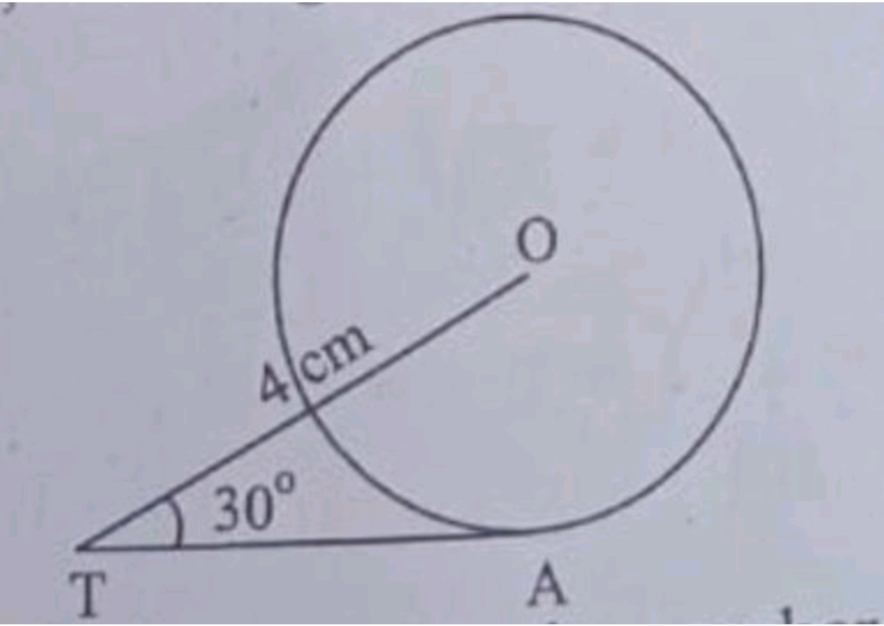
\includegraphics[width=\columnwidth]{figs/image 1.jpg}
\label{fig:image1}
	\caption{image1}
\end{figure}
\item In the given figure,$\triangle ABC \sim \triangle QPR$,If $AC = 6\mathrm{cm},BC = 5 \mathrm{cm},QR = 3\mathrm{cm}  and PR = x$;then the value of  x is:
	\begin{enumerate}
	\item $3.6 \mathrm{cm}$
	\item $2.5\mathrm{cm}$
	\item $10 \mathrm{cm}$
	\item $3.2 \mathrm{cm}$
	\end{enumerate}
	\begin{figure}[!ht]
\centering
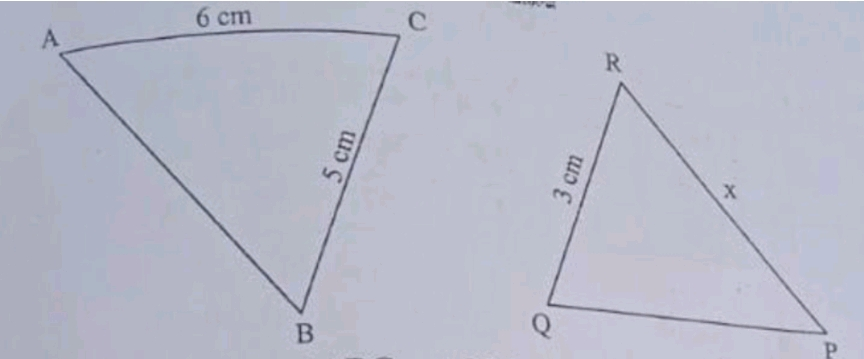
\includegraphics[width=\columnwidth]{figs/image 2.jpg}
\label{fig:image1}
	\caption{image2}
\end{figure}
\item The distance of the point $\brak{-6,8}$ from origin is:
	\begin{enumerate}
	\item $6$
	\item $-6$
	\item $8$
	\item $10$
\end{enumerate}
\item What is the area of a semi-circle of diameter $\brak{d}$?
\begin{enumerate}
    \item $\frac{1}{16} \times \pi \times d^2$
    \item $\frac{1}{4} \times \pi \times d^2$
    \item $\frac{1}{8} \times \pi \times d^2$
    \item $\frac{1}{2} \times \pi \times d^2$
\end{enumerate}
\item In the given figure, $PT$ is a tangent at $T$ to the circle with centre $\brak{o}$. If $\angle TPO = 25\degree$, then $x$ is equal to:
\begin{figure}[!ht]
\centering
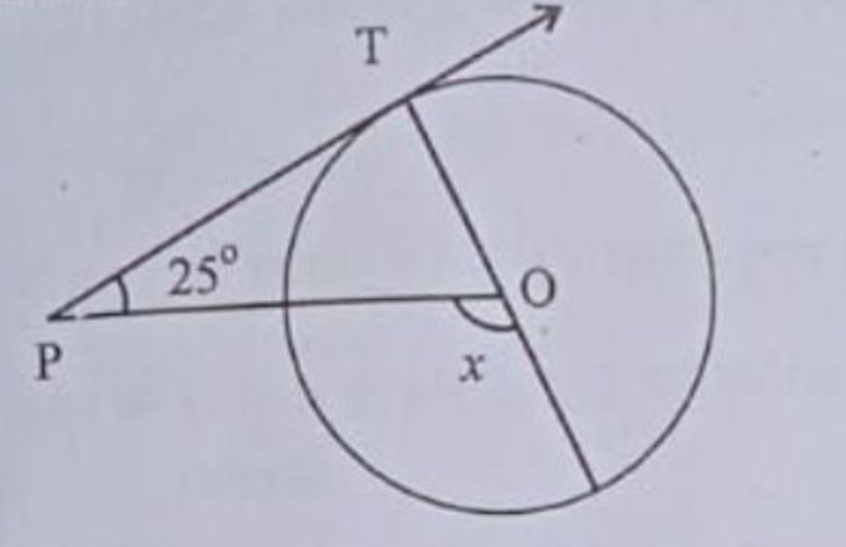
\includegraphics[width=\columnwidth]{figs/image 3.jpg}
\label{fig:image1}
        \caption{image3}
\end{figure}
\begin{enumerate}
    \item $25\degree$
    \item $65\degree$
    \item $90\degree$
    \item $115\degree$
\end{enumerate}
\newpage
\item In the given figure, $PQ \parallel AC$. If $BP = 4 \, \mathrm{cm}$, $AP = 2.4 \mathrm{cm}$, and $BQ = 5 \, \mathrm{cm}$, then the length of $BC$ is:
\begin{figure}[!ht]
\centering
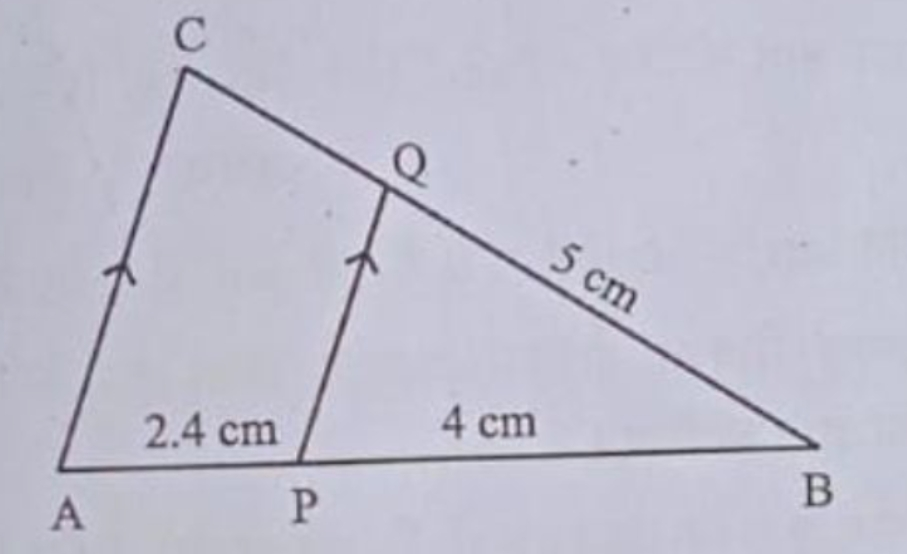
\includegraphics[width=\columnwidth]{figs/image 4.jpg}
\label{fig:image1}                                                  \caption{image4}                                    
\end{figure}
	\begin{enumerate}
    \item $8\mathrm{cm}$
    \item $3\mathrm{cm}$
    \item $0.3 \mathrm{cm}$
    \item $\frac{25}{3}\mathrm{cm}$
\end{enumerate}
\item The points $\brak{-4,0},\brak {4,0}, and \brak{0,3}$ are the vertices of a:

\begin{enumerate}
    \item right triangle
    \item isosceles triangle
    \item equilateral triangle
    \item scalene triangle
\end{enumerate}


\item What is the length of the arc of the sector of a circle with radius $14\mathrm{cm}$ and a central angle of $90\degree$:    
\begin{enumerate}
\item  $ 22\mathrm{cm} $  
\item  $ 44\mathrm{cm} $
\item  $ 88\mathrm{cm}$                                            
\item  $ 11\mathrm{cm}$
\end{enumerate}


\item If $\triangle ABC  \triangle PQR$ with $\angle A = 32\degree $ and $\angle R = 65\degree$, then the measure of $\angle B$ is?:
\begin{enumerate}
\item $ 32\degree $                                                
\item $ 65\degree $                                            
\item $ 83\degree $                                
\item $ 97\degree $
\end{enumerate}


\item  The coordinates of vertex A of a triangle ABCD whose three vertices are given as $B\brak{0,0}$, $C\brak{3,0}$, and $D\brak{0,4}$ are?:  
    \begin{enumerate}
    \item $  \brak{4,0} $                      
    \item $  \brak{0,3} $                          
    \item $  \brak{3,4} $                                  
    \item $  \brak{5,3} $
    \end{enumerate}
    \item The area of the triangle formed by the line axes is: $\frac{x}{a} +\frac{y}{b} = 1$ with the coordinate axes is:  
    \begin{enumerate}
    \item $ ab $                                    
    \item $ \frac{1}{2}ab $        
    \item $ \frac{1}{4}ab $              
    \item $ 2ab $
    \end{enumerate}

item In the given figure, $DE \parallel BC$. If $AD = 2 units$, $DB = AE =3 units$ and $EC = x units$, then the value of $x$ is:                                                                
\begin{figure}[h!]
\centering                                            
	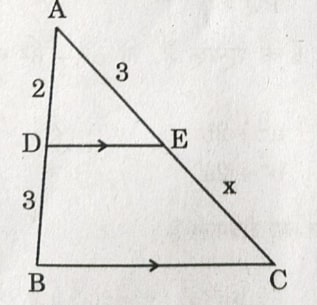
\includegraphics[width=\columnwidth]{figs/t1.jpg}    
\label{fig:image1}                                
\end{figure}
\begin{enumerate}
\item $ 2 $                                                          
\item $ 3 $                    
\item $ 5 $                                      
\item $ \frac{9}{2} $
\end{enumerate}
\newpage
\item In the given figure, $AB \parallel PQ$. If $AB = 6\mathrm{cm}$, $PQ =   2\mathrm{cm} $and $OB = 3\mathrm{cm}$, then the length of $OP$ is:
\begin{figure}[h!]      
\centering
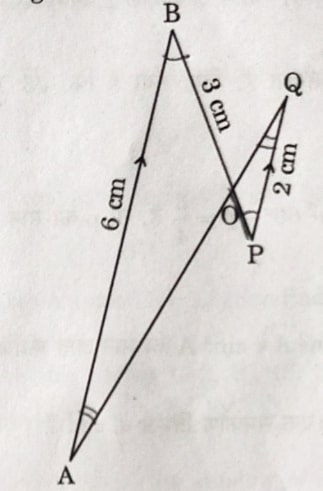
\includegraphics[width=\columnwidth]{figs/t2.jpg}  
\label{fig:image3}                              
\end{figure}
\begin{enumerate}
\item $ 9\mathrm{cm} $                                      
\item $ 3\mathrm{cm} $        
\item $ 4\mathrm{cm} $                                    
\item $ 1\mathrm{cm} $  
\end{enumerate}

\item What Is The Total Surface Area Of a Solid Hemisphere Of Diameter 'd'?:   
	\begin{enumerate}                          
    \item $ 3\pi d^2 $                        
    \item $ 2\pi d^2 $                                    
    \item $ \frac{1}{2}\pi d^2 $
    \item $ \frac{3}{4}\pi d^2 $
    \end{enumerate}
 
\item
From an external point, two tangents are drawn to a circle. Prove that the line joining the external point to the center of the circle bisects the angle between the two tangents.
\item
	Two concentric circles are of radii $5\mathrm{cm}$and $3\mathrm{cm}$. Find the length of the chord of the larger circle which touches the smaller circle.
\item
In a $\triangle{PQR}$, $N$ is a point on $PR$, such that $QN$$\perp$$PR$. If $PN \times NR=QN^2$, prove that $\angle{PQR}=90^{\circ}$.
\newpage
\item
In the given figure, $\triangle ABC$  and  $\triangle$ $DBC$  are on the same base $BC$.  $AD$ intersects $BC$ at $O$.
prove that  $\frac{\text{ar}\brak{\triangle ABC}}{\text{ar}\brak{\triangle DBC}} = \frac{AO}{DO}$
\begin{figure}[h!]
\centering
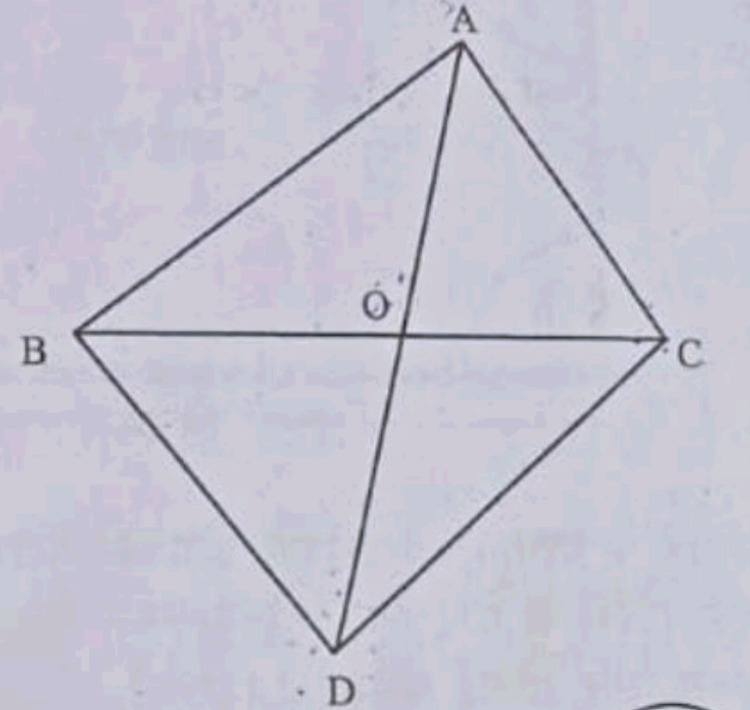
\includegraphics[width=\columnwidth]{figs/img1.jpg}
\caption{Image 1}
\end{figure} 
\newpage
\item
	A wooden article was made by scooping out a hemisphere from each end of a solid cylinder, as shown in the figure. If the height of the cylinder is $10\mathrm{cm}$ and its base is of radius $3.5\mathrm{cm}$, find the total surface area of the article.
\begin{figure}[h!]
\centering
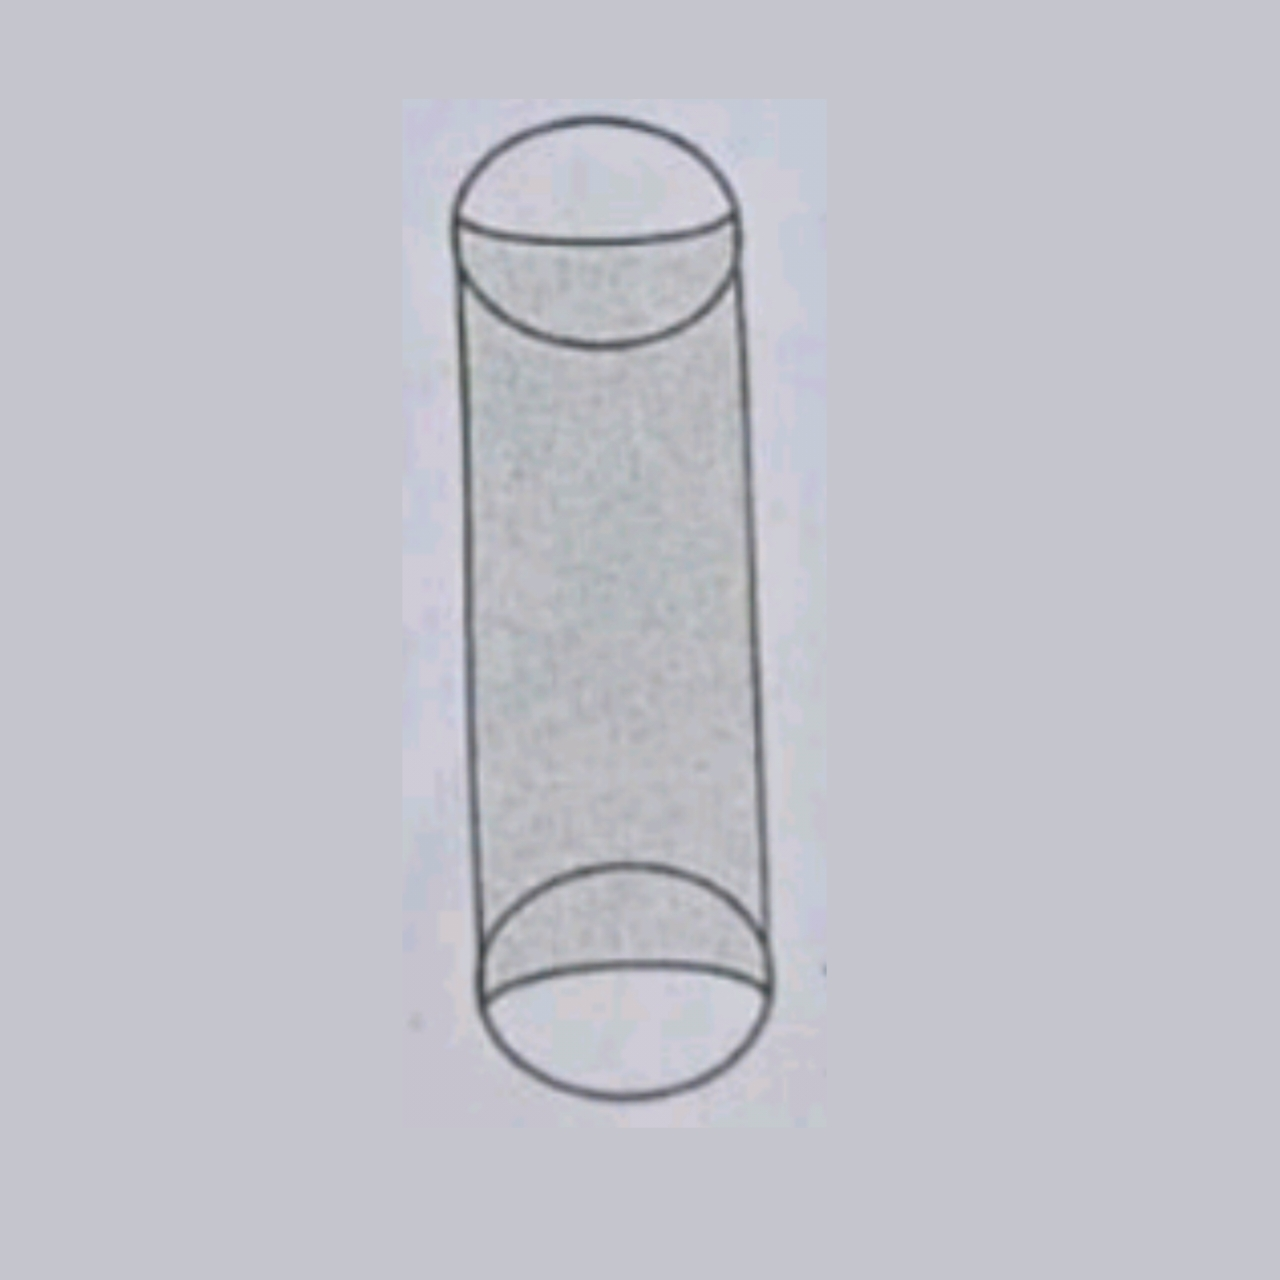
\includegraphics[width=\columnwidth]{figs/img2.jpg}
\caption{Image 2}
\end{figure}
\newpage
\item
Governing council of a local publc development authority of Dehradun decided to build an adventurous playground on the top of a hill, which will have adequate space for parking.
\begin{figure}[h!]
\centering
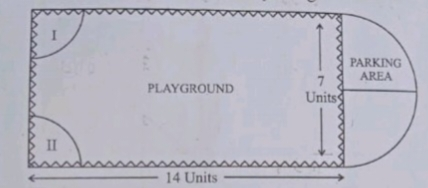
\includegraphics[width=\columnwidth]{figs/img3.jpg}
\caption{Image 3}
\end{figure}
After survey, it was decide to build rectangular playground, with a semi-circular area allotted for parking at one one end of the playground. The length and breadth of the rectangular playground are $14$ units and $7$ units, respectively. There are two quadrants of radius $2$ units on one side for s
pecial seats.
Based on the above information, answer the following questions:
\begin{enumerate}
\item
What is the total perimeter of the parking area?
\item
\begin{enumerate}
\item
What is the total area of parking and the two quadrants?
\item
Whast is the ratio of area of playground to the area of paarking area?
\end{enumerate}
\item
Find the cost of fencing the playground and parking area at the rate of \rupee $2$ per unit.
\newpage
\item
Two schools $P$ and $Q$ decided to award prizes to their students for two games of Hockey \rupee $x$ per student and Cricket \rupee $y$ per student. School $P$ decided to award a total of \rupee $9,500$ for the two games to $5$ and $4$ students respectively; while school $Q$ decided to award
 \rupee $7,370$ for the two games to $4$ and $3$ students respectively.
\begin{figure}[h!]
\centering
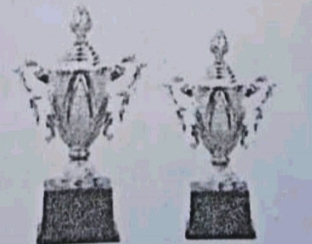
\includegraphics[width=\columnwidth]{figs/img4.jpg}
\caption{Image 4}
\end{figure}
Based on the given information,answer the following questions:
\begin{enumerate}
\item
Represent the following information in algebraically (in terms of $x$ and $y$).
\item
\begin{enumerate}
\item
What is the prize amount for hockey?
\item
Prize amount on which game is more and by how much?
\end{enumerate}
\item
What will be the total prize amount if there are $2$ students each from two games?
\end{enumerate}
\end{enumerate}
\newpage
\item
Jagadish has a field which is in the shape of a right angled triangle $AQC$. He wants to leave a space in the form of a square $PQRS$ inside the field for growing wheat and the remaining for growing vegetables \brak{as shown in the figure}. In the field, there is a pole marked as $O$.
\begin{figure}[h!]
\centering
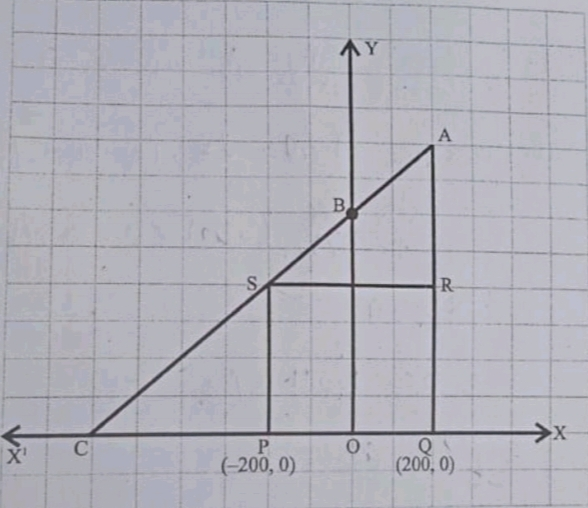
\includegraphics[width=\columnwidth]{figs/img5.jpg}
\caption{Image 5}
\end{figure}
Based on the above information, answer the following questions:
\begin{enumerate}
\item
Taking $O$ as origin, coordinates of $P$ are \brak{-200,0} and of $Q$ are \brak{200,0}. $PQRS$ being a square, what are the coordinates of $R$ and $S$?
\item
\begin{enumerate}
\item
What is the area of square $PQRS$?
\item
What is the length of diagonal $PR$ in square $PQRS$?
\end{enumerate}
\item
If $S$ divides $CA$ in the ratio $K:1$, what is the value of $K$, where point $A$ is \brak{200,800}?
\end{enumerate}

\end{enumerate}

